\section{Reference solution approach}
As the aim of this work is to prepare a universally usable solver for MHD problems, the refinement indicator \Cref{refinementIndicator} must ideally not be dependent on any attributes of the solved problem data (initial condition, boundary conditions, physical quantities such as $\gamma$, etc.). In order to achieve this, the so-called{reference solution} approach is used.
\paragraph{}
The reference solution approach is not only problem, but also equation (physics) independent, which is truly invaluable for many types of physical problems, even so for multi-physics coupled problems, such as MHD.
\subsection{Algorithm}
Algorithm, given in \Cref{AMRRef} is accompanied by an example in \Crefrange{figure:amrRef1}{figure:amrRef16}:\ \\
\begin{algorithm}[H]
\label{AMRRef}
 \KwData{Mesh $T_0$}
 \KwResult{A mesh $T_n$ and a solution $\bfy_n$ on this mesh satisfying the solution acceptance criteria}
 i = 0\\
 \While{true}{
  obtain solution $\bfy_i$ on $T_i$\\
	evaluate solution $\bfy_i$ acceptance criteria\\
	\eIf{solution acceptance criteria satisfied} {
		return\\
   } {
		identify subset $T^{r}_i$ of all elements $K \in T_i$ to be refined, $T^{r}_i \subseteq T_i$\\
		obtain $T_{i+1}$ by refining (at least) all $K \in T^{r}_i$\\
		i = i + 1\\
	}
 }
 \caption{Generic AMR algorithm}
\end{algorithm}

\begin{figure}[H]
	\begin{center}
%		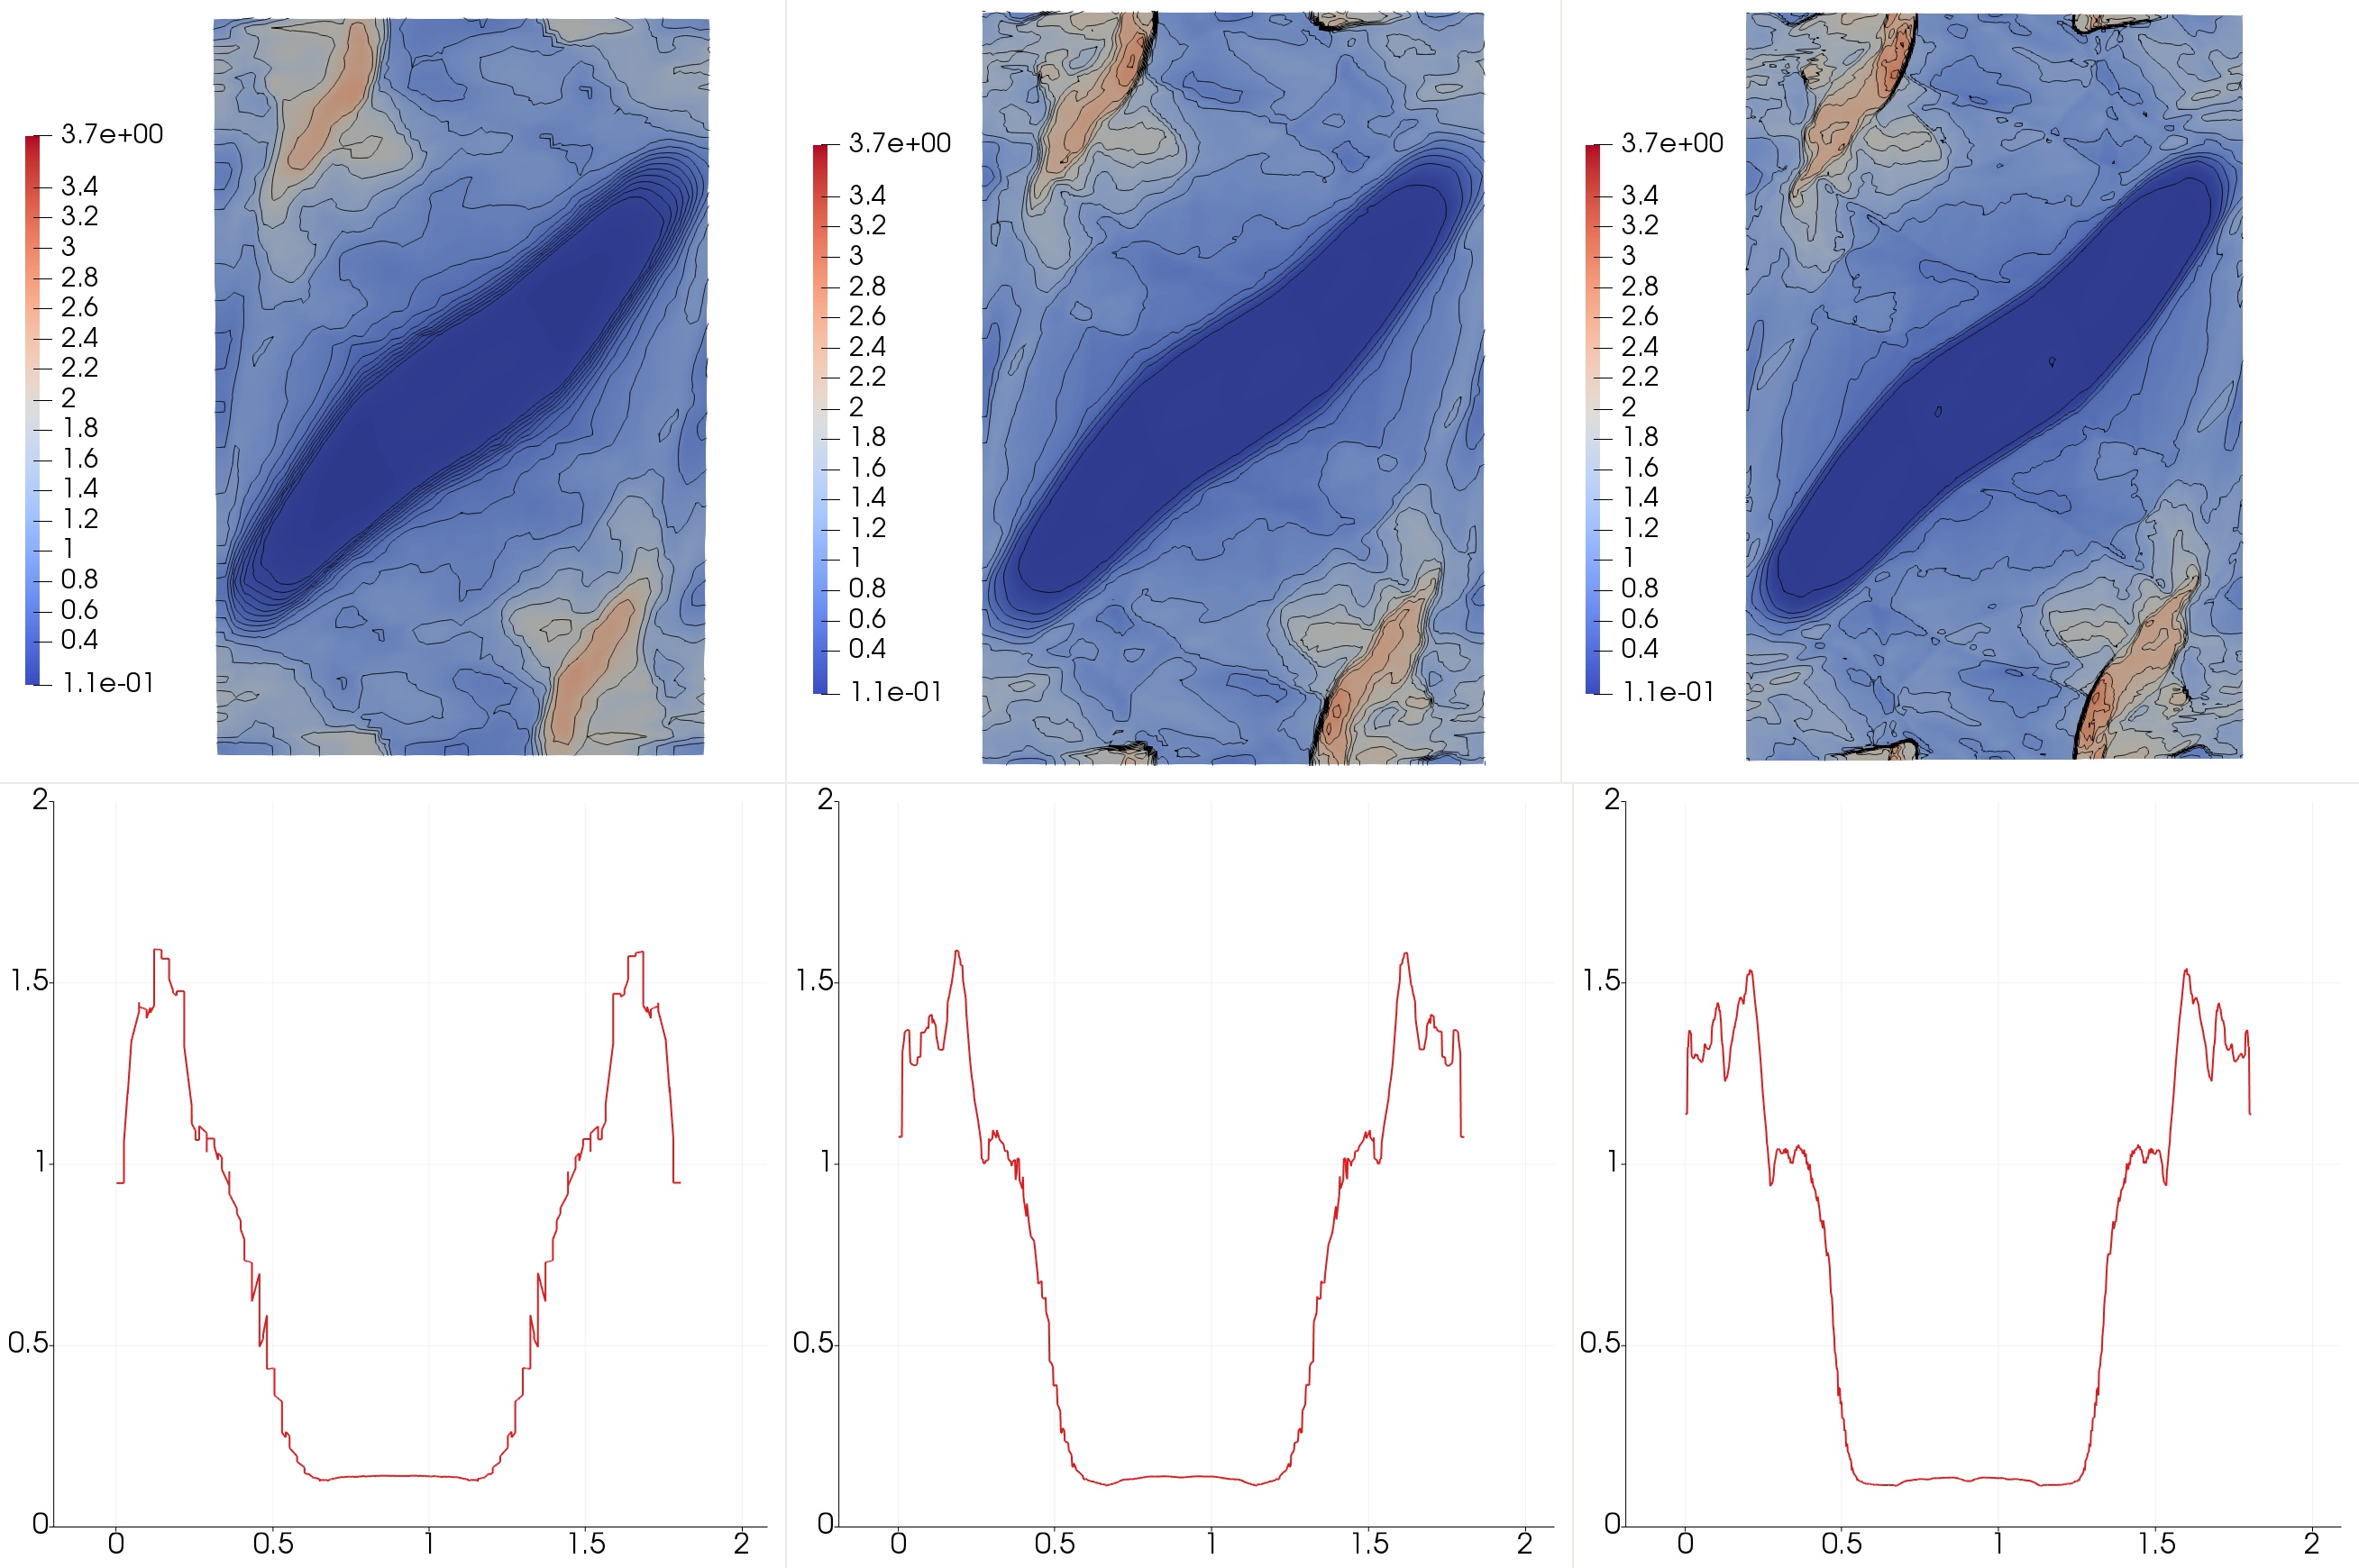
\includegraphics[width=0.92\textwidth]{img/mhd-blast/new/blast,1noadapt18.jpg}
		\caption{Fine solution on mesh }
	\label{figure:amrRef1}
	\end{center}
\end{figure}
\vspace{-4mm}


TODO - add outputs (Hermes / deal)
TODO - ukazat na 2d prikladu z Hermesu co to je referencni reseni, co to je ||zprojektovane - presne|| (v dealu?), co to je tohle bez normy, zminka o distribuovanosti, ze musim napocitat nejaky thresholdy mapReducem, atd.
